\documentclass[12pt]{exam}

% LOAD PACKAGES
\usepackage{amsmath} % allows for align env and other things
\usepackage{amssymb} % 
\usepackage{mathtools} % allows for single apostrophe
\usepackage{enumitem} % allows for alpha lettering in enumerated lists
\usepackage{lastpage}
\usepackage{array} % for table alignments
\usepackage{graphicx} % if images are needed

\addpoints

% Initials
\newcommand{\Initials}{\textit{\Course, \TestName. Your initials: \underline{\hspace{3cm}}} \vspace{1pt}}
\newcommand{\InitialsLeft}{\noindent \hspace{-18pt}\textit{\Course, \TestName. Your initials: \underline{\hspace{3cm}}} \vspace{1pt}}
\newcommand{\InitialsRight}{\begin{flushright}\textit{\Course, \TestName. Your initials: \underline{\hspace{3cm}}} \vspace{1pt}\end{flushright}}


% INSTRUCTIONS FOR DISTANCE LEARNING COURSES: PROCTORS/FACILITATORS
\newcommand{\InstructionsDistanceProctors}{\begin{itemize}

    \item A proctor/facilitator is required to be present while the student is taking this test.
    
    \item A proctor/facilitator must connect with the on-campus class during this test.   
        
    \item For any connection help: gtonlinesupport@pe.gatech.edu
    
    \item No communication is allowed among students taking the exam.

\end{itemize}}


% INSTRUCTIONS FOR DISTANCE LEARNING COURSES: STUDENTS
\newcommand{\InstructionsDistanceStudents}{\begin{itemize} \setlength\itemsep{.15em}
    
    % \item If there are questions during the exam, students can call/text \InstructorContact, at \InstructorNumber, under supervision of their proctor/facilitator.     
        
    \item {\bf Show your work} and justify your answers for all questions unless stated otherwise.

    \item You will have \Duration continuous minutes (no breaks) to take the exam. 
    
    \item There are \Points total points possible.

    \item Calculators, notes, cell phones, books are not allowed.
    
    \item Please write your answers neatly and show all of your work. 
    \item Use dark and clear writing: your exam will be scanned into a digital system.
    
    \item Exam pages are double sided. Be sure to complete both sides. 
    
    \item Leave a 1 inch border around the edges of exams.
    
    \item Check that every page has the same booklet number.

\end{itemize}}


% INSTRUCTIONS FOR DISTANCE LEARNING COURSES: STUDENTS
\newcommand{\InstructionsCovid}{\begin{itemize} \setlength\itemsep{.15em}
    
    \item If there are questions during the exam, students can email their instructor or message them through Canvas. 
    
    % \InstructorContact, at \InstructorNumber, under supervision of their proctor/facilitator.     
        
    \item {\bf Show your work} and justify your answers for all questions unless stated otherwise.

    \item You will have \Duration continuous minutes (no breaks) to take the exam. 
    
    \item There are \Points total points possible.
    
    \item Your work must be your own. Please do not communicate with anyone other than the instructor during the exam. Otherwise, students can use any resources available to them the answer the questions that are given. 
    
    \item Students can take this exam at home.
    
    \item Please write your answers neatly and show all of your work. 
    
    \item Students should scan their work and submit it through Canvas. There should be an \textbf{assignment} in Canvas for this exam. The process for submitting your work will be similar to what you have used for homework. 
    
    \item Work must be submitted today by 12:30 ET. 
    
    \item Please use dark and clear writing so that the scan is easy to read. 
    
    \item Please write your name or initials at the top of every page and solve the questions in the exam in the order they are given. 
    
    \item There is no need to print the exam at home. As long as you solve problems in the order they are given (just like the written homework sets), you can write out your work on your own paper. But of course, you can print the exam out if you prefer and write your answers on the printed copy. 
    
    \item Please upload your work as a single PDF file. If this is not possible you can email your work to your instructor. 


    
\end{itemize}}

% FANCY HEADERS - MAKE EMPTY
\pagestyle{headandfoot}
\runningfooter{}{}{}


% ADJUST MARGINS FOR DISTANCE LEARNING REQUIREMENTS
\usepackage[tmargin=1.7in,bmargin=1.05in,left=1in,right=1in]{geometry}


% TIKZ DIAGRAMS
\usepackage{color}
\usepackage{tikz}  \usetikzlibrary{arrows} 
\usetikzlibrary{calc} 


% ADJUST FIRST LINE IN PARAGRAPH INDENTATION 
\setlength\parindent{0pt}


% COURSE SPECIFIC INFORMATION
\newcommand{\Course}{Math 2552}
\newcommand{\Semester}{Spring}
\newcommand{\Year}{2020}
\newcommand{\Instructors}{Dr. Greg Mayer}

% WHO TO CONTACT DURING EXAM IF QUESTIONS
\newcommand{\InstructorContact}{Dr. Greg Mayer}


\usepackage{spalign} % Joe Rabinoff's matrix package

\newcommand{\LastPage}{\begin{center}\textit{This page may be used for scratch work. Please indicate clearly if you would like your work on this page to be graded. }\end{center}   }

\newcommand{\Scratch}{\begin{center}\textit{This page may be used for scratch work for the previous question. Your proctor should scan this page whether it is used or not. }\end{center}   }


% DERIVATIVES
\newcommand{\dydt}{{\frac{dy}{dt}}} % 
\newcommand{\dydx}{{\frac{dy}{dx}}} % 
\newcommand{\dydtt}{{\frac{d ^2y}{dt^2}}} % 
\newcommand{\dydxx}{{\frac{d^2y}{dx^2}}} % 
\newcommand{\dydttt}{{\frac{d^3y}{dt^3}}} % 

\newcommand{\ddt}{{\frac{d}{dt}}} % 
\newcommand{\ddx}{{\frac{d}{dx}}} % 
\newcommand{\dudt}{{\frac{du}{dt}}} % 
\newcommand{\dvdx}{{\frac{dv}{dx}}} % 
\newcommand{\dxdt}{{\frac{dx}{dt}}} % 
\newcommand{\dxdtt}{{\frac{d^2x}{dt^2}}} % 
\newcommand{\dzdt}{{\frac{dz}{dt}}} % 



% TEST SPECIFIC INFORMATION
\newcommand{\TestName}{Sample Midterm 1A}
\newcommand{\TestDate}{May 2019}
\newcommand{\TestTime}{10:05 am to 11:20 am}
\newcommand{\Duration}{75 \ }
\newcommand{\Points}{50 \ }


\begin{document}
    
% % create space for QR Code (crowdmark)
\vspace*{-1cm}

\begin{center}
{\Large \TestName, \Course, \Semester \ \Year}
\end{center}

\begin{center}    
{\small
Instructor: \Instructors \\ Please administer \TestDate. Students should have 50 minutes to take this exam. 
}
\end{center}

\begin{center} 
    \textbf{PLEASE DO NOT PHOTOCOPY THIS EXAM} \\[8pt]
    {\small 
    High School:  \underline{\hspace{4cm}}, GT Email Address: \underline{\hspace{4cm} @gatech.edu} 
    }
\end{center}

% % HONOR CODE
% \vspace{6pt}
% \textbf{Georgia Tech Honor Code}\\
% {\footnotesize \GTHonorCode}

% \begin{center}
% \begin{center}
%     \def\arraystretch{0.35}%  1 is the default, change whatever you need
%     \begin{tabular}{ b{8cm} b{8cm} }
%     \vspace{.5cm} \underline{\hspace{7cm}} & \vspace{.5cm} \underline{\hspace{4.5cm}}  \tabularnewline
%     \vspace{6pt} signature & \vspace{6pt} date    
%     \end{tabular}
% \end{center}
% \end{center}

\vspace{9cm}

% INSTRUCTIONS FOR STUDENTS
\vspace{12pt}
\textbf{Student Instructions}
{\small \InstructionsDistanceStudents}



\newpage

\textit{On your midterm, each question below would be given one page.} 

\begin{questions}

%  ~ ~ ~ ~  ~ ~ ~ ~  ~ ~ ~ ~  ~ ~ ~ ~  ~ ~ ~ ~  ~ ~ ~ ~

\question[10] Solve the following initial value problems. You may leave your answers as implicit relations in $t$ and $y$. 

   \begin{parts} 
    
        \part $\displaystyle y\dydt = (t + ty^2)e^{t^2}, \quad y(0) = 2$
        
        \part $\displaystyle t^3 \dydt + 4t^2 y = e^{-t}, \quad t < 0, \quad y(-1) = 0$
        
    \end{parts}

\question[10] Suppose $A = \spalignmat{-3 2; 1 1}.$  % based on 3.4 # 10
 	
   \begin{parts} 
    
        \part Determine the eigenvalues of $A$.

        \part Determine the eigenvectors of $A$. 

        \part Express the general solution of the system $\vec x \, ' = A \vec x$ in terms of real valued functions. 
        
        \part Sketch the phase portrait of the system.         
        
    \end{parts}
 	
    \question[4] A tank holds 500 litres of salt water. Initially, there are 0.5 kg of salt in the tank. Salt water containing 3 kg of salt per litre is pumped into the tank at a rate of 4 litres per minute. The well mixed solution is pumped out at a rate of 2 litres per minute. Construct an initial value problem that models the amount of salt in the tank for $t\in[0,T]$, where $T$ is some positive constant. Do not solve your initial value problem. 

    \question[3] Transform the equation $\displaystyle 2y'' + 4 y' + 8ty = 12t^2$ into an equivalent first order system. 

    \question[3] % 
    Suppose $\vec x \, ' = A \vec x$, where $A$ is the $2\times 2$ matrix
    $A = \spalignmat{0,-4;4,0}$.
    The eigenvalues of $A$ are $\pm 4i$. Sketch the phase portrait. Label your axes.
    \question[4] An amount $S_0$ is invested at an annual rate of return $r$ percent, compounded continuously. Determine the number of years required for the original investment to double in value, as a function of $r$. 
    \question[6] Consider the system $$ \vec x \, ' = A \vec x = \spalignmat{-1 -4;1 -1} \vec x$$ The eigenvalues of $A$ are $\lambda = -1 \pm 2i$. 
    \begin{enumerate}
        \item Determine the eigenvectors of $A$. 
        \item Write down the solution to the linear system. 
        \item Classify the critical point(s) of the system in terms of stability and type.
    \end{enumerate}
    \question[10] Consider the differential equation $\displaystyle \dydt = 3y^2 - 2y^3$.
    \begin{parts}
        \part Indicate the equilibrium solutions.
        \part Sketch the phase line and classify the equilibrium solutions. 
        \part Determine where $y$ is concave up and where it is concave down.
        \part Use the information you obtained in parts (a), (b), and (c) to sketch a few integral curves. 
    
    \end{parts}    
    

\end{questions}

\newpage

\large{Answers}

\begin{enumerate}
    \item 
    \begin{enumerate}
        \item This question based on 2.1 \# 7. Separable: 
    \begin{align*}
        \frac{y}{1+y^2} dy &= te^{t^2} dt \\
        \int \frac{y}{1+y^2} dy &= \int te^{t^2} dt + C, \quad \text{set } u = t^2, du = 2t dt \\
        \frac12 \ln (1+y^2) &= \frac12 \int e^u du + C \\
         \ln (1+y^2) &= e^{t^2} + C \\
        y(0) = 2: \quad \ln (1 + 2) &= e^0 + C \quad \Rightarrow \quad C = \ln 3 - e \\
        \ln( 1 + y^2) &= e^{t^2} + \ln 3 - e
    \end{align*}
    \item This is question 2.2 \#19. If you have been working through the recommended homework exercises you should have the solution. The solution to the differential equation with arbitrary constant $c_1$ is $$y = c_1t^{-4} - t^{-4} e^{-t} - t^{-3}e^{-t}$$
    We were given that $y(-1) = 0$, so
    \begin{align*}
        0 &= c_1(-1)^{-4} - (-1)^{-4} e^{1} - (-1)^{-3}e^{1} \\
        0 &= c_1 - e + e \\
        c_1 &= 0
    \end{align*}
    The solution to the initial value problem (IVP) is
    $$y = - t^{-4} e^{-t} - t^{-3}e^{-t}$$
    
    \end{enumerate}
    \item Solution on next page. 
    
    
    % \begin{enumerate}
    %     \item Characteristic polynomial: 
    %     \begin{align*}
    %         0 &= (-3 - \lambda) (1 - \lambda) - 2 \\
    %         &= \lambda^2 +2\lambda - 5 \\
    %         \lambda &= -1 \pm \frac12 \sqrt{4+20} = -1 \pm \sqrt{6}
    %     \end{align*}
    %     \item \begin{align*}
    %         A - (-1 \pm \sqrt{6}) I = \begin{pmatrix} -2\mp\sqrt{6} & 2 \\ \ast & \ast \end{pmatrix}
    %     \end{align*}
    %     $\ast$ = not needed because $A-\lambda I$ is singular. The first row gives us $(-2 \mp \sqrt6)x_1 + 2x_2 = 0$. If $x_1 = 2$, then $x_2 = 2 \pm \sqrt6$. Eigenvectors are: 
    %     $$\vec v_1 = \spalignmat{2;2+\sqrt6}, \vec v_2 = \spalignmat{2;2-\sqrt6}$$
    %     \item $\displaystyle \vec x(t) = c_1 e^{-1+\sqrt6 t}\spalignmat{2;2+\sqrt6} + c_2e^{-1-\sqrt6 t}\spalignmat{2;2-\sqrt6} $
    %     \item Labeling axes and arrows along trajectories are important. Sketch on next page. 
    %     \newpage 
    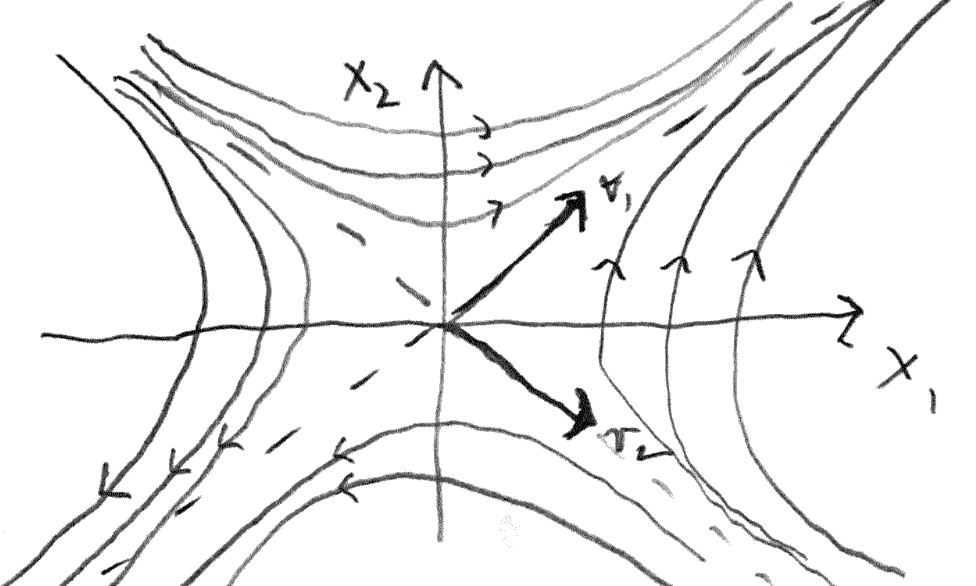
\includegraphics[scale=1.5]{./PhasePortrait2.png}
    % \end{enumerate}
    
    \newpage
    
    \item \begin{align*}
        Q'(t) &= \text{(rate in) - (rate out)} \\ 
        &= 3\cdot4 - 2\frac{Q}{500+2t} \\
        &= 12 - \frac{Q}{250+t}, \quad Q(0) = \frac12, \quad t \in [0,T]
    \end{align*}
    \item Let 
    \begin{align*}
        x_1 &= y \\
        x_2 &= y' 
    \end{align*}
    Then 
    \begin{align*}
        x_1' &= x_2 \\
        x_2' &= y'' = 6t^2 - 2x_2 - 4tx_1
    \end{align*}
    As a matrix equation we have
    \begin{align*}
        \vec x \, ' (t) = \spalignmat{x_1';x_2'} = \spalignmat{0 1;-4t -2}\vec x + \spalignmat{0;6t^2}
    \end{align*}
    
    \item Solution on next page. 
    
    \newpage
    
    \item This is question 2.3 \# 10. 
    \begin{align*}
        S' &= r S \\ 
        S &= S_0e^{rt} \\
        2S_0 &= S_0e^{rT} \\
        T &= \frac 1r \ln 2
    \end{align*}
    \item This is based on a question from section 3.4, \# 7. 
    \begin{enumerate}
        \item The eigenvectors are $\spalignmat{\pm2i;1}=\spalignmat{0;1}+ i\spalignmat{\pm2;0}$.
        \item From the eigenvectors and eigenvalues, we have the solution $$\vec x (t) = e^{-t} \left( \spalignmat{0;1}\cos2t - \spalignmat{2;0 } \right)\sin2t + i e^{-t}\left( \spalignmat{0;1}\sin2t + \spalignmat{2;0 }\cos2t \right)$$
        \item The only critical point is at $(0,0)$ and the critical point is an asymptotically stable spiral sink.
    \end{enumerate}
    \item Solution on next page. 
\end{enumerate}

\end{document}


